\section{Design and implementation}

In this section the considerations for the
design will be discussed. This includes the overall design for the application
as well as the problems that the individual features posed. The section also
details how the proposed solutions were carried out and implemented in the
application.

\subsection{Overall design}
%Jonas
\subsubsection{Design patterns}

Mvvm, wpf, data bindings Model assembly

\subsubsection{Function list}
Based on the requirements and the definition of UML class 
diagrams\footnote{http://en.wikipedia.org/wiki/Class\_diagram} 
\footnote{http://www.digilife.be/quickreferences/qrc/uml quick reference 
card.pdf}, a function list is produced.

\begin{table}[H]
	\begin{tabular}{lll}
		\hline
		\textbf{Ribbon: File menu} 
		&                                                                       
		                     &
		                                                                        
		             \\ \hline
		New                        & \begin{tabular}[c]{@{}l@{}}Create new 
		project\\ Close/discard open project\end{tabular}    & 
		Ctrl+Shift+N                                                            
		            \\
		Open                       & Open existing 
		project                                                                 
		     &
		 
		Ctrl+O                                                                  
		            \\
		Save                       & Save current 
		project                                                                 
		      &
		 
		Ctrl+S                                                                  
		            \\
		Save As                    & Save current project as new 
		file                                                           & 
		Ctrl+Alt+S                                                              
		            \\
		Print                      & Print 
		diagram                                                                 
		             &
		 
		Ctrl+P                                                                  
		            \\
		Export                     & Export project to 
		PNG                                                                     
		 &
		 
		Ctrl+E                                                                  
		            \\
		 \hline
		&                                                                       
		                     
		&                                                                       
		              \\
		 \hline
		\textbf{Ribbon: Edit}      
		&                                                                       
		                     &
		                                                                        
		             \\ \hline
		Undo                       & Undo previous 
		actions                                                                 
		     &
		 
		Ctrl+Z                                                                  
		            \\
		Redo                       & Redo 
		actions                                                                 
		              &
		 
		Ctrl+Shift+Z                                                            
		            \\
		Paste                      & Paste class from 
		clipboard                                                               
		  &
		 
		Ctrl+V                                                                  
		            \\
		Cut                        & Cut 
		class                                                                   
		               &
		 
		Ctrl+X                                                                  
		            \\
		Copy                       & Copy selected 
		class                                                                   
		     &
		 
		Ctrl+C                                                                  
		            \\
		New Class                  & Add 
		class                                                                   
		               &
		 
		Ctrl+N                                                                  
		            \\
		Delete Class               & Delete selected 
		class                                                                   
		   &
		 
		Delete                                                                  
		            \\
		Relations                  & \begin{tabular}[c]{@{}l@{}}Add relation 
		between classes\\ (enter add mode)\end{tabular}    
		&                                                                       
		              \\
		Delete relation            & \begin{tabular}[c]{@{}l@{}}Delete 
		relation\\ (show circle, enter delete mode)\end{tabular} 
		&                                                                       
		              \\
		 \hline
		&                                                                       
		                     
		&                                                                       
		              \\
		 \hline
		\textbf{Canvas functions}  
		&                                                                       
		                     &
		                                                                        
		             \\ \hline
		Select class               
		&                                                                       
		                     &
		 Click on 
		class                                                                   
		   \\
		Drag class                 
		&                                                                       
		                     &
		 Drag class with 
		mouse                                                               \\
		Add relation               & (during add relation 
		mode)                                                                 & 
		\begin{tabular}[c]{@{}l@{}}Click on class "from"\\ Click on class 
		"to"\end{tabular} \\
		Delete relation            & (during delete relation 
		mode)                                                              & 
		\begin{tabular}[c]{@{}l@{}}Click on relation\\ 
		(circle)\end{tabular}                \\
		Change class name          
		&                                                                       
		                     &
		 Click on text 
		field                                                                 \\
		Add field / method         
		&                                                                       
		                     &
		 Click 
		+                                                                       
		      \\
		Remove field / method      
		&                                                                       
		                     &
		 Click 
		X                                                                       
		      \\
		Edit field/method text     
		&                                                                       
		                     &
		 Click on text 
		field                                                                 \\
		Edit relation text         
		&                                                                       
		                     &
		 Click on text 
		field                                                                 \\
		 \hline
	\end{tabular}
\end{table}

\subsection{Graphichal User interface}

\subsubsection{Design}

Even though that
user interface design was not a main scope of the project, some thought is
required as it greatly impacts the user experience. 

The overall decision to make it wether to whether to use an existing design
framework, or to create a whole new layout with toolbars, menues etc. Since it
is not in the scope of the project and the benefit would be minimal it was
decided to go with an already tested and know interface. 

The traditional Windows application is defined by its layered menus and toobars,
which execls at more complicated programs where submenus are essential.

The other viable alternative is the
\textit{Ribbon}\footnote{http://msdn.microsoft.com/en-us/library/windows/desktop/dd316910(v=vs.85).aspx}
framework which is know for its big toolbar with the most used functions ready
for use.

Based on the original program mockup as previously seen in figure \ref{mockup},
it was clear that all the menu items could be in such a bar that the Ribbon
interface offers without creating additional layers.

It also seemed a good fit for a graphical editing tool, as the Ribbon interface
has an emphasis on having a graphical display for each action. This makes the
tool a lot easier to use for new users, as for example a relation could be
accompanied by a graphical representation showing exactly how the relation will
look like.

\subsubsection{Implementation} 
The \textit{GUI} was created with \texttt{XAML} and the standard windows
\textit{Ribbon} API. \texttt{XAML} supports defining all the graphical elements,
but also data bindings and user events.

\paragraph{Classes and relations}
The classes are composed of a class name, and an area where the
fields and methods go. Each class can have an arbitrary number of fields and
methods. The
amount is controlled by the green plus sign and the red delete sign.

The relations consist of a line between two classes, and an "arrowhead" which
denotes the type of relation. Although not shown in the sceenshot all relations
also has a textfield which can be used to show multiplicity.

An example with three classes and some relations can be seen in figure
\ref{classes}. This also shows how the program is composed of a canvas and a
toolbar.

\begin{figure}[H]
\centering
\includegraphics[width=\linewidth]{"img/example"}
\caption{Classes and Relations \label{classes}}
\end{figure}


\paragraph{Ribbon Toolbar}
The ribbon toolbar features all the most used functions. Our toolbar can be seen in
figure \ref{toolbar}. The actions are
structured into \textit{Clipboard \& history}, \textit{Classes},
\textit{Relations}. As a feature of the ribbon toolbar, each action can also be
reached by using a hotkey, which can be seen when holding the ALT key.

\begin{figure}[H]
\centering
\includegraphics[width=\linewidth]{"img/edit menu"}
\caption{Ribbon Toolbar \label{toolbar}}
\end{figure}

\paragraph{Menu}
The main menu is mainly used for actions which interacts with files, such as
loading or saving diagrams. Also more advanced features such as exporting is put
here.

\begin{figure}[H]
\centering
\includegraphics[width=\linewidth]{"img/file menu"}
\caption{File Menu \label{menu}}
\end{figure}

\subsection{Application}
In this part the application part of the program is discussed.

\subsubsection{Klasses and relations}
%Jonas
The \texttt{Klass} and \texttt{Relation} classes are the backbone of the model.
So they were put in their own \texttt{dll}. This ensures reusability, and makes
the program more flexible, in that it does not consist of 1 giant exe file.

\paragraph{Klass}
The \texttt{Klass} class is the representation of a class in any object oriented
language. The class contains almost all the info a class should have. Some of
the missing stuff is interfaces and abstract classes, but these can be added in
future iterations.

The class also contains some of the info needed to render it properly, such as
an $(x, y)$ coordinate as well as such things as height, width, and some color
properties. Some of this probably belongs in a viewmodel class but we found it
easier to just implement it directly in this class instead.

The consequence of having viewmodel properties in the model, was that
\texttt{Klass} also had to have a list of all the relations that was hooked up
to it. This was to be able to notify any relation whenever a \texttt{Klass} is
moved in the GUI. 

What became easier from having the viewmodel properties in the model, was the
serialization, and how to handle the relation between \texttt{Klass} and
\texttt{Relation}. Having a relation between the 2 models, and 2 viewmodels
would make it hard to maintain the right state.

\paragraph{Relation}
The \texttt{Relation} class is used to represent the relation in a UML diagram.
This class has to be flexible to allow for many different types of relations,
such as inheritance, reference, composition, etc. The class uses an enum to
know
which type of relation it is. This eliminates the need to create a new subclass
every time a new type of relation is introduced.

The \texttt{Relation} class, is basically just a class that holds 2
\texttt{Klass} classes. This makes it possible to draw a line between these 2
classes.

The relation is drawn using the 3rd party library called
LineCaps\footnote{http://blogs.msdn.com/b/mrochon/archive/2011/01/10/custom-line-caps-in-wpf.aspx}.

The library made it possible to easily add the shapes that represents different
types of relations e.g. a diamond for the composition, to the ends of the line.
DataTriggers was added to the style property of the view. These DataTriggers was
then set to trigger on the type property of the \texttt{Relation}, making a new
style for each type.

\subsubsection{Saving \& loading}
The save and open functionality is based on the serialization process. Objects
can be serialized to a sequence of bytes either as binary data or in an XML
structure. The serialized data can be stored in a file, and loaded into the
application later by deserializing the objects.

For this project, two solutions were considered. Using the functionality in the
\texttt{System.Runtime.Serialization} namespace, or using the XmlSerializer
class from the \texttt{System.Xml.Serialization} namespace. The Runtime
Serialization allows us to store the serialized objects as binary data or
formatted as SOAP data.

The three options all have their advantages and disadvantages. We have chosen
runtime serialization with binary formatting, based on what we found as
described in the following sections.

\paragraph{XML Serializer}

The XmlSerializer class provides easy to use
functionality to serialize and deserialize simple objects to an XML format. It
is possible to define which objects are serializable, and which field of objects
that should be serialized, and which should not.

However, the XmlSerializer class, does not support references to objects. This
means, that every time the serializer meets a serializable object, the object
will be serialized - even though it may already have done so. This does not
allow for cyclic references, which we have in our program. In our case, a Klass
object references a list of Relations, which in turn references a To and From
Klass.

If we were to use the XmlSerializer class, we would have to change the structure
of our program.

\paragraph{Runtime serialization}

The classes in the runtime serialization
namespace supports references to objects. When the serializer meets an object,
which has already been serialized, the object is referenced and not
re-serialized.

%TODO: ISerializable… 

The runtime serialization allows for two types of formatting: Binary and SOAP.

\textbf{Binary formatting}\\
Binary formatting serializes the objects to a
sequence of bytes, which is unreadable to humans. It works, but it has the
disadvantage, that it can be hard to verify, that the serializer does what it is
meant to do.

\textbf{SOAP formatting}\\
SOAP is a protocol used to exchange information, and
is often used in web services which provide data to other applications through
an API. The resulting data when using SOAP formatting is an XML structure,
similar to the structur of the XmlSerializer and iis more friendly to human
interpretation than its binary counterpart.

However, for some reason, the SOAP formatter attempted to serialize objects from
our MVVM libray, even though it was not told to, which made the serialization
fail.

\paragraph{Save \& open dialogs}
To allow the user to save and open diagram files, the standard save- and open 
file dialog boxes are utilized. This functionality allows us to define which 
files the user should see; in our case \emph{.dia} files.

\begin{figure}[H]
	\centering
	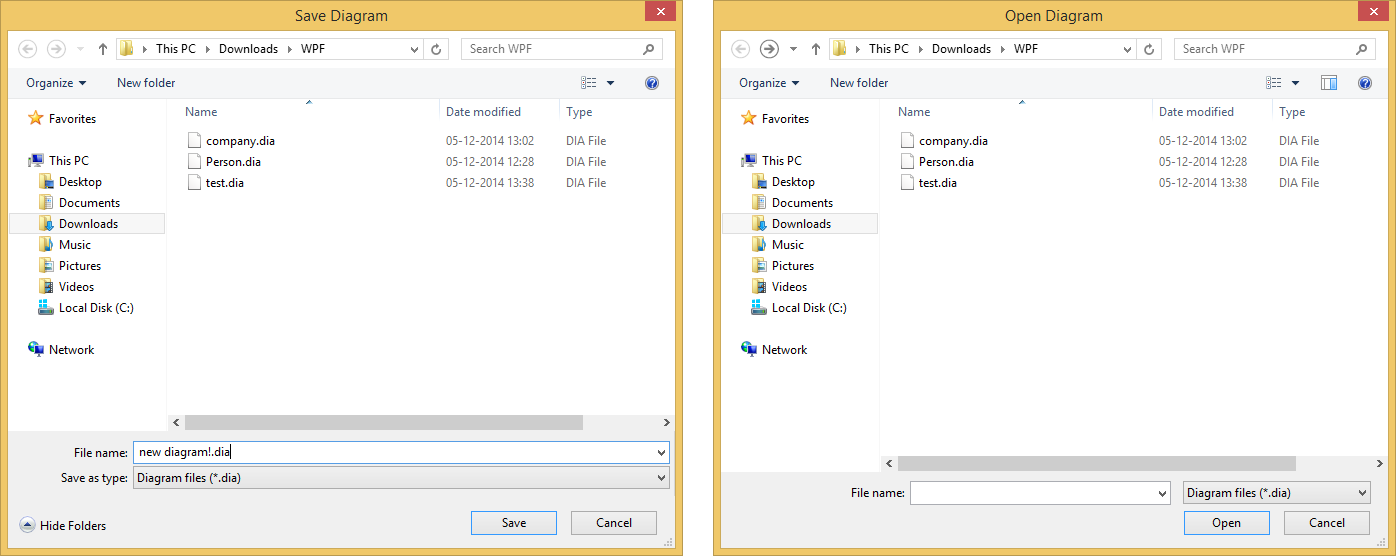
\includegraphics[width=\linewidth]{img/save_open.png}
	\caption{Save and open dialog boxes \label{saveopen}}
\end{figure}

\subsubsection{Using threads}
Serialization, deserialization and reading/writing
to files are processes that might take some time for the computer to execute.
Thus, threads can be used to improve the user experience by preventing the
window from “freezing” while these processes are going on. Typically, the
diagrams made in this program are relatively small and simple, and the user may
not notice anything when saving and opening without threads. However, the
difference may be noticeable if the users hard drive is really slow, or the
diagram is really big.

In our case, the saving process is handled by a thread, which allows the user to
continue working while the objects are saved in the background. Opening files
are not executed in a thread, since the user should wait for everything to be
loaded anyway. It could easily be implemented, but the save functionality
exemplifies the process quite well.


\subsubsection{Undo / Redo}
%Peter
All commands supporting the undo/redo functionality implments the
IUndoRedoCommand interface, which extends ICommand. The singleton class
UndoRedoController handles the undo- and redo-stacks, which keep track of the
previous states of the application. All UndoRedoCommands are executed through
the AddAndExecute methods, of this class.

The applications enables undo/redo functionality on the following actions:


\begin{itemize}
	\item New class
	\item Delete class
	\item Add relation
	\item Delete relation
	\item Cut
	\item Paste
	\item Move class
\end{itemize}


\subsubsection{Copy, cut \& paste}

A simple clipboard is implemented in the
application to allow copying, cutting and pasting classes. When pasting a class
from the clipboard, the class and its content (fields and methods) are copied,
but not its relations. This behaviour is intended, as we believe that this is
the typical use case for copy/paste.

The clipboard functionality utilizes the existing commands for deleting and
creating new classes, hence, it also supports the undo/redo functionality of
those.

%TODO: Noget om at copy paste på text ikke virker?
This solution only supports copy paste of class objects. If it made sense, this 
could be extended to support additional objects. The implementation does not 
overwrite the built in clipboard of Windows. Thus, the user can still 
copy/paste text from and to text fields within the application.

\subsubsection{Image export}

To make it easier for the users to use the created diagram, an image export tool
was implemented. Only support for \textit{png} was implemented as it it
the most suited filetype for this kind of graphics. An important thing to consider
is how to ensure that only the relevant part of the canvas it exported, so
the users does't have to crop the image later.

\texttt{Export} was implemented in the \texttt{MainViewModel}, by creating a
\texttt{RelayCommand} that takes the canvas as argument.
The \texttt{Export} method then finds all the  descendants bounds, which is 
the minimum area that ensures that all relevant elements are exported. The
default renderer however always renders from $(0,0)$, so an auxiliary method to
cancel this offset was used. The standard Windows Save dialog was used toi
select the image path.

